\section{Marco conceptual}
\label{sec:marco_conceptual}
En esta sección se presentan conceptos y bases teóricas respecto a la temática que conduce el desarrollo de este trabajo, el cual tiene relación con el uso de interfaces no tradicionales, específicamente con una interfaz operada con el cuerpo. Además, se indaga sobre ciertas definiciones para establecer lo que se pretende medir en este estudio, lo que involucra la experiencia de usuario y métricas de rendimiento en la realización de tareas. Finalmente, se proponen ciertas características fundamentales respecto de este tipo de proyectos relacionados con diseños experimentales con usuarios.

\ingles{Human Computer Information Retrieval} (HCIR) o Recuperación de Información Humano 
Computador\footnote{Traducción libre.}, es el estudio de los métodos que integran la inteligencia humana y la búsqueda algorítmica para ayudar a la gente a mejorar la búsqueda, exploración y aprendizaje de información (Marchionini, 2007). Dentro de esta área interactúan otras disciplinas, como la recuperación de información, llamada en inglés \ingles{Information Retrieval} (IR), la que está enfocada principalmente en proveer a los usuarios de fácil acceso a la información de su interés trabajando con la representación, almacenamiento, organización y acceso a objetos de información como documentos, páginas \ingles{web}, catálogos en línea y objetos multimedia (Baeza-Yates & Ribeiro-Neto, 2011) y la búsqueda de información, llamada en inglés \ingles{Information Seeking} (IS) que se entiende como un proceso más orientado al usuario y abierto que IR. En IS, no se sabe si existe una respuesta a la consulta del usuario, por lo que el proceso de búsqueda puede proporcionar el aprendizaje necesario para satisfacer su necesidad de información (Baeza-Yates & Ribeiro-Neto, 2011). 

\subsection{Búsqueda de información}
\label{subsec:busqueda}

\subsection{Rendimiento}
\label{subsec:rendimiento}
En el contexto de la recuperación de información se definen \ingles{precision} y \ingles{recall} en función de un conjunto de documentos relevantes y un conjunto de documentos recuperados (Powers, 2011), las cuales se definen a continuación.  

\begin{description}
	\item [\ingles{Precision}] Métrica que mide la razón de documentos relevantes recuperados con 
respecto al total de documentos recuperados. Es un valor continuo entre 0 y 1, mientras más cercano a 1, mayor fue su precisión al encontrar los documentos relevantes.
	\begin{equation}
	Precision = \frac{\big[\big\{documentos \ relevantes\big\} \cap \big\{documentos \ recuperados\big\}\big]}{\big\{documentos \ recuperados\big\}}
	\end{equation}

	\item [\ingles{Recall}] Métrica que mide la razón de documentos relevantes recuperados con 
respecto al total de documentos relevantes. Es un valor continuo entre 0 y 1, mientras más cercano a 1, mayor fue la recuperación de documentos en base al total del universo disponible.
	\begin{equation}
	Recall = \frac{\big[\big\{documentos \ relevantes\big\} \cap \big\{documentos \ recuperados\big\}\big]}{\big\{documentos \ relevantes\big\}}
	\end{equation}

	\item [\ingles{F1}] Métrica que considera a \ingles{precision} y \ingles{recall} en un promedio ponderado. Es un valor continuo entre 0 y 1, en que un valor cercano a uno permite identificar a los estudiantes con una recuperación de documentos proporcional a su precisión, respecto a la relevancia de estos.   
	\begin{equation}
	F1 = \frac{2 \cdot Precision\cdot Recall}{Precision+ Recall}
	\end{equation}
 
	\item [\ingles{Coverage Effectiveness}] Razón entre la cobertura útil, páginas visitadas sobre 30 segundos, y el total de documentos visitados por un estudiante. Es un valor continuo entre 0 a 1, mientras más cercano a 1, mejor fue la efectividad de la cobertura respecto el universo de documentos, respecto al tiempo de permanencia.     
	\begin{equation}
	CE = \frac{UsfCover}{TotalCover}
	\end{equation}

	\item [\ingles{Query Effectiveness}] Razón existente entre la efectividad de la cobertura (fórmula anterior) y el total de consultas realizadas por un estudiante. Esta proporción da indicios del desempeño del estudiante en torno a la calidad de las consultas efectuadas, en base a la cantidad y eficacia. Sus valores también están en un intervalo continuo entre 0 a 1.
	\begin{equation}
	QE = \frac{CE}{countQ}
	\end{equation}

	\item [\ingles{Search Score}] Calificación de los estudiantes que se expresa en una escala continua de 0 a 5 puntos. Es una razón entre la cobertura relevante y el total de páginas marcadas activas al final de la tarea. 
	\begin{equation}
	Score = \frac{BMRelv}{ActBM} * 5
	\end{equation}

\end{description}

%\begin{equation}
%	Precision = \frac{TP}{TP+ FP}
%\end{equation}
%\begin{equation}
%	Recall = \frac{TP}{TP+ FN}
%\end{equation}
\subsection{Alfabetización informacional}
\label{subsec:alfabetizacion}
La alfabetización informacional (conocida en ingles \ingles{information literacy}) es definida como “el grupo de habilidades en las que se requiere reconocer cuándo la información es necesaria y tener la habilidad de encontrar, evaluar y usar efectivamente dicha información necesaria” \footnote{\traduccionlibre} \parencite[p.~2]{american2000information}. Es un campo que cubre varias áreas, entre las que se destaca la alfabetización digital, las habilidades de uso de bibliotecas, la ética informacional, la lectura crítica, el pensamiento crítico, los derechos de autor, la seguridad y privacidad, entre otras. A través del estudio de estas áreas como factores que influyen a la alfabetización informacional se puede obtener una visión clara de cómo los estudiantes llevan a cabo sus tareas de obtención y selección de información.

\subsection{Competencias de investigación en línea}
\label{subsec:competencias}
Se definen las competencias de investigación (\ingles{inquiry skills} en inglés) como “las habilidades para explorar preguntas, para poder reunir, interpretar y sintetizar diferentes tipos de información y datos, además de desarrollar y compartir una explicación para responder preguntas dadas” \footnote{\traduccionlibre} \parencite[p.~13]{national2000inquiry}. En base a este concepto nacen las competencias de investigación en línea (conocidas en inglés como \ingles{online inquiry skills}), que son una instancia específica de las competencias de investigación, pero aplicada sobre información disponible en línea \parencite{quintana2005framework}.

Las competencias de investigación en línea involucran una serie de actividades cognitivas, como generar una pregunta de investigación, buscar información relevante en colecciones digitales, evaluar y seleccionar la información encontrada, e integrar coherentemente la información seleccionada para responder la pregunta original \parencite{eisenberg1990information}.

\subsection{Minería de datos educacional}
La minería de datos utiliza una combinación de bases de conocimientos explícita, conocimientos analíticos complejos y conocimiento de campo para descubrir las tendencias y los patrones ocultos, estas tendencias y patrones forman la base de los modelos predictivos que permiten a los analistas realizar nuevas observaciones de los datos existentes \parencite{luan2002data}. La gran cantidad de información generada hoy en día por los estudiantes permite que la minería de datos obtenga datos relevantes y, a través de métodos estadísticos y otras herramientas, relacione la información para conocer si el proceso de enseñanza aprendizaje ha dado resultados positivos. 

\textcite[p.~9]{mining2012enhancing} define la minería de datos educacional (MDE, desde ahora en adelante) como “la teoría que desarrolla métodos, aplica técnicas estadísticas y de aprendizaje automático para analizar los datos recogidos durante el proceso de la enseñanza y aprendizaje” \footnote{\traduccionlibre}. Actualmente, los usos más generales que se le están dando a la MDE básicamente se enfocan en mejorar la estructura del conocimiento y determinar el apoyo pedagógico al estudiante.

\subsection{Técnicas de minería de datos}
\label{subsec:tecnicas-mineria}

\subsection*{\ingles{Support Vector Machine}}

\begin{figure}[H]
	\centering
	\begin{tikzpicture}[&gt;=stealth']
  % Draw axes
  \draw [&lt;-&gt;,thick] (0,5) node (yaxis) [above] {$y$}
        |- (5,0) node (xaxis) [right] {$x$};
  % draw line
  \draw (0,-1) -- (5,4); % y=x-1
  \draw[dashed] (-1,0) -- (4,5); % y=x+1
  \draw[dashed] (2,-1) -- (6,3); % y=x-3
  % \draw labels
  \draw (3.5,3) node[rotate=45,font=\small] 
        {$\mathbf{w}\cdot \mathbf{x} + b = 0$};
  \draw (2.5,4) node[rotate=45,font=\small] 
        {$\mathbf{w}\cdot \mathbf{x} + b > 1$};
  \draw (4.5,2) node[rotate=45,font=\small] 
        {$\mathbf{w}\cdot \mathbf{x} + b < -1$};
  % draw distance
  \draw[dotted] (4,5) -- (6,3);
  \draw (5.25,4.25) node[rotate=-45] {$\frac{2}{\Vert \mathbf{w} \Vert}$};
  \draw[dotted] (0,0) -- (0.5,-0.5);
  \draw (0,-0.5) node[rotate=-45] {$\frac{b}{\Vert \mathbf{w} \Vert}$};
  \draw[-&gt;] (2,1) -- (1.5,1.5);
  \draw (1.85,1.35) node[rotate=-45] {$\mathbf{w}$};
  % draw negative dots
  \fill[red] (0.5,1.5) circle (3pt);
  \fill[red]   (1.5,2.5)   circle (3pt);
  \fill[black] (1,2.5)     circle (3pt);
  \fill[black] (0.75,2)    circle (3pt);
  \fill[black] (0.6,1.9)   circle (3pt);
  \fill[black] (0.77, 2.5) circle (3pt);
  \fill[black] (1.5,3)     circle (3pt);
  \fill[black] (1.3,3.3)   circle (3pt);
  \fill[black] (0.6,3.2)   circle (3pt);
  % draw positive dots
  \draw[red,thick] (4,1)     circle (3pt); 
  \draw[red,thick] (3.3,.3)  circle (3pt); 
  \draw[black]     (4.5,1.2) circle (3pt); 
  \draw[black]     (4.5,.5)  circle (3pt); 
  \draw[black]     (3.9,.7)  circle (3pt); 
  \draw[black]     (5,1)     circle (3pt); 
  \draw[black]     (3.5,.2)  circle (3pt); 
  \draw[black]     (4,.3)    circle (3pt); 
\end{tikzpicture}
	\captionsource{SVM}{\fuentePropia}
	\label{fig:svm}
\end{figure}

\subsection*{Perceptrón multicapa}

\begin{figure}[H]
	\centering
	% Multilayer perceptron
\usetikzlibrary{positioning}

\tikzstyle{inputNode}=[draw,circle,minimum size=10pt,inner sep=0pt]
\tikzstyle{stateTransition}=[-stealth, thick]

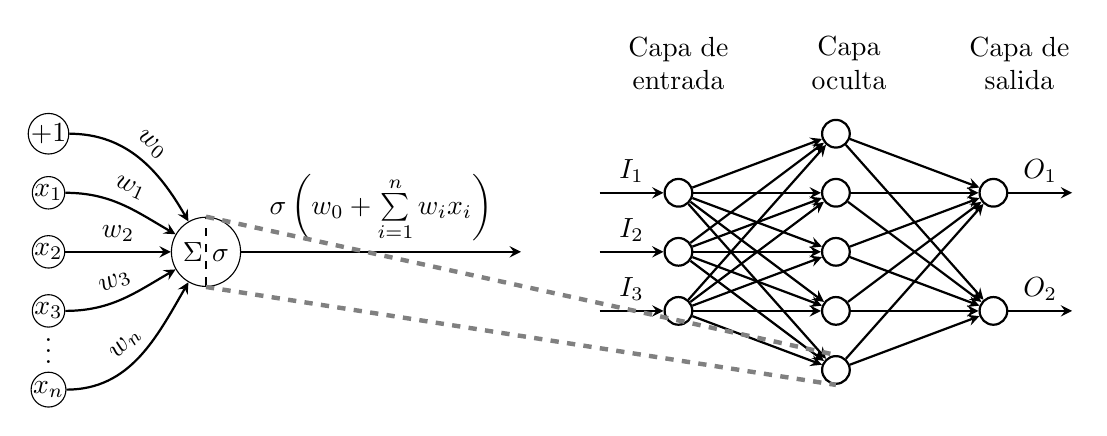
\begin{tikzpicture}
    \node[draw,circle,minimum size=25pt,inner sep=0pt] (x) at (0,0) {$\Sigma$ $\sigma$};

    \node[inputNode] (x0) at (-2, 1.5) {$\tiny +1$};
    \node[inputNode] (x1) at (-2, 0.75) {$\tiny x_1$};
    \node[inputNode] (x2) at (-2, 0) {$\tiny x_2$};
    \node[inputNode] (x3) at (-2, -0.75) {$\tiny x_3$};
    \node[inputNode] (xn) at (-2, -1.75) {$\tiny x_n$};

    \draw[stateTransition] (x0) to[out=0,in=120] node [midway, sloped, above] {$w_0$} (x);
    \draw[stateTransition] (x1) to[out=0,in=150] node [midway, sloped, above] {$w_1$} (x);
    \draw[stateTransition] (x2) to[out=0,in=180] node [midway, sloped, above] {$w_2$} (x);
    \draw[stateTransition] (x3) to[out=0,in=210] node [midway, sloped, above] {$w_3$} (x);
    \draw[stateTransition] (xn) to[out=0,in=240] node [midway, sloped, above] {$w_n$} (x);
    \draw[stateTransition] (x) -- (4,0) node [midway,above] {$\sigma\left(w_0 + \sum\limits_{i=1}^{n}{w_ix_i}\right)$};
    \draw[dashed] (0,-0.43) -- (0,0.43);
    \node (dots) at (-2, -1.15) {$\vdots$};
    \node[inputNode, thick] (i1) at (6, 0.75) {};
    \node[inputNode, thick] (i2) at (6, 0) {};
    \node[inputNode, thick] (i3) at (6, -0.75) {};
    
    \node[inputNode, thick] (h1) at (8, 1.5) {};
    \node[inputNode, thick] (h2) at (8, 0.75) {};
    \node[inputNode, thick] (h3) at (8, 0) {};
    \node[inputNode, thick] (h4) at (8, -0.75) {};
    \node[inputNode, thick] (h5) at (8, -1.5) {};
    
    \node[inputNode, thick] (o1) at (10, 0.75) {};
    \node[inputNode, thick] (o2) at (10, -0.75) {};
    
    \draw[stateTransition] (5, 0.75) -- node[above] {$I_1$} (i1);
    \draw[stateTransition] (5, 0) -- node[above] {$I_2$} (i2);
    \draw[stateTransition] (5, -0.75) -- node[above] {$I_3$} (i3);
    
    \draw[stateTransition] (i1) -- (h1);
    \draw[stateTransition] (i1) -- (h2);
    \draw[stateTransition] (i1) -- (h3);
    \draw[stateTransition] (i1) -- (h4);
    \draw[stateTransition] (i1) -- (h5);
    \draw[stateTransition] (i2) -- (h1);
    \draw[stateTransition] (i2) -- (h2);
    \draw[stateTransition] (i2) -- (h3);
    \draw[stateTransition] (i2) -- (h4);
    \draw[stateTransition] (i2) -- (h5);
    \draw[stateTransition] (i3) -- (h1);
    \draw[stateTransition] (i3) -- (h2);
    \draw[stateTransition] (i3) -- (h3);
    \draw[stateTransition] (i3) -- (h4);
    \draw[stateTransition] (i3) -- (h5);
    
    \draw[stateTransition] (h1) -- (o1);
    \draw[stateTransition] (h1) -- (o2);
    \draw[stateTransition] (h2) -- (o1);
    \draw[stateTransition] (h2) -- (o2);
    \draw[stateTransition] (h3) -- (o1);
    \draw[stateTransition] (h3) -- (o2);
    \draw[stateTransition] (h4) -- (o1);
    \draw[stateTransition] (h4) -- (o2);
    \draw[stateTransition] (h5) -- (o1);
    \draw[stateTransition] (h5) -- (o2);
    
    %Input layer
    \node[above=of i1, align=center] (l1) {Capa de \\ entrada};
    %Hidden Layer
    \node[right=2.3em of l1, align=center] (l2) {Capa \\ oculta};
    %Output Layer
    \node[right=2.3em of l2, align=center] (l3) {Capa de \\ salida};
    
    \draw[stateTransition] (o1) -- node[above] {$O_1$} (11, 0.75);
    \draw[stateTransition] (o2) -- node[above] {$O_2$} (11, -0.75);
    
    \path[dashed, double, ultra thick, gray] (x.north) edge[bend left=0] (h5.north);
    \path[dashed, double, ultra thick, gray] (x.south) edge[bend right=0] (h5.south);
\end{tikzpicture}

	\captionsource{Perceptrón multicapa}{\fuentePropia}
	\label{fig:multilayer-perceptron}
\end{figure}